\documentclass{../base/base}
% Dateikodierung ist utf8
\usepackage[utf8]{inputenc}
\usepackage{url}
\usepackage[export]{adjustbox}
\usepackage{amsmath}
\usepackage{listings}
\usepackage{tikz}
\usepackage{tabularx}
\usepackage{color,colortbl}
\usepackage{ulem}
\usepackage{pdfpages}
\usepackage{ wasysym }
\usepackage{ booktabs }
\usepackage{lscape}
\usepackage{multicol}

\begin{document}

\Abgabeblatt{Assignment 1}{16.03.2018}{????}{????}{Yannis Rohloff (yannis@uni-bremen.de)}{Liu Meng(lium@uni-bremen.de)}{Peter Tschubij (tschupet@uni-bremen.de)}

\lstset{
    language=Python,
    basicstyle=\ttfamily\small,
    aboveskip={1.0\baselineskip},
    belowskip={1.0\baselineskip},
    columns=fixed,
    extendedchars=true,
    breaklines=true,
    tabsize=4,
    prebreak=\raisebox{0ex}[0ex][0ex]{\ensuremath{\hookleftarrow}},
    frame=lines,
    showtabs=false,
    showspaces=false,
    showstringspaces=false,
    keywordstyle=\color[rgb]{0.627,0.126,0.941},
    commentstyle=\color[rgb]{0.133,0.545,0.133},
    stringstyle=\color[rgb]{01,0,0},
    numbers=left,
    numberstyle=\small,
    stepnumber=1,
    numbersep=10pt,
    captionpos=t,
    escapeinside={\%*}{*)}
}


\section{Graph Coloring}
The following Python script was used to generate the CNF and encode it into the neccesary .cnf format.

\subsection{Vertex Coloring}
\subsubsection{petersen.py:}
\lstinputlisting{petersen.py}

This file was used to generate the petersen.cnf on the following page.

The script records comments and clauses into a list and counts the clauses. The amount of clauses is needed on the first line of the .cnf output.
We iterate over the 3 defined constraints from the course. This is basically just translating the big conjunctions into for loops.


The cnf generated by this program is in petersen.cnf

\subsubsection{picosat solution of petersen.cnf:}
The picosat output gives the following solution:
\lstinputlisting{petersen.solution}
with the variables meaning:
\lstinputlisting{petersen.vars}

By reading the meaning of the numbers in in the last comments of the petersen.cnf we can color the graph like this:\\ \\
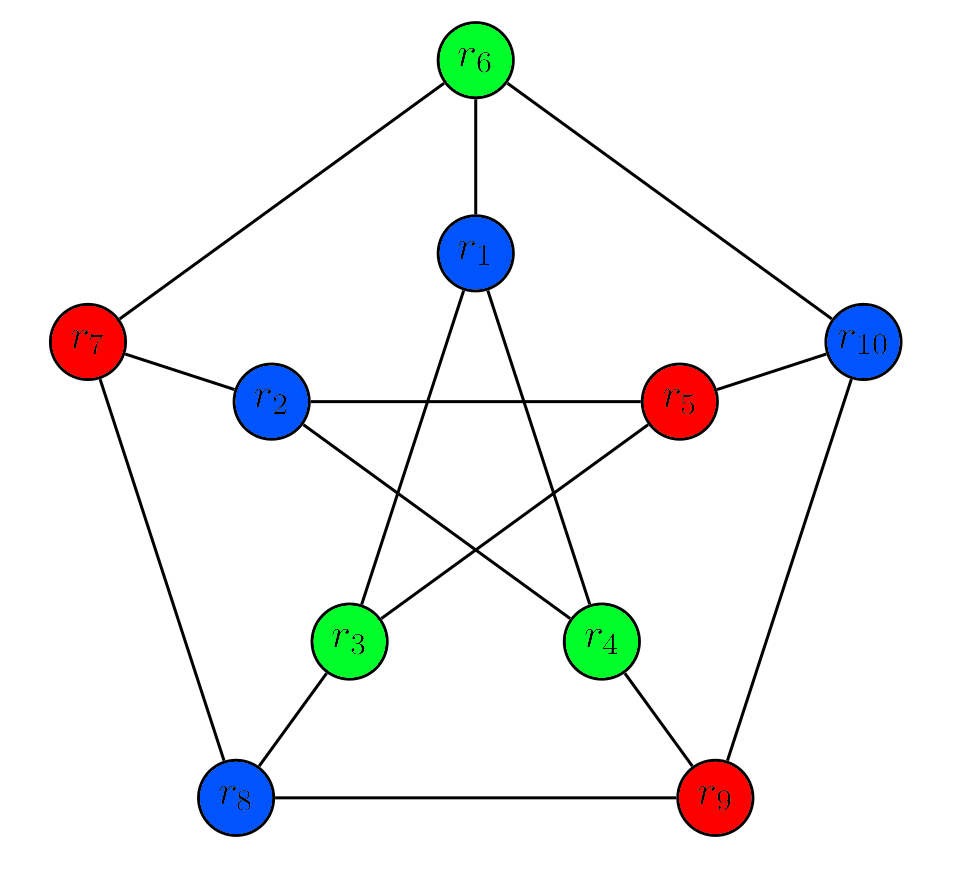
\includegraphics[width=10cm]{petersen_colored.png}


\clearpage
\subsection{Edge Coloring}
To transform the Vertex Coloring Sat Constraints into constraints that describe the $n$-Edge Coloring problem we only need to make a few changes. The new Constraints can be defined as shown below:


First for Graph $G = (V,E)$ and Colors $C =\{0,\dots,n\}$, we define a variable $x_{abc}$ for each edge $(a,b) \in E$ and color $c \in C$ variables for each edge.


\textbf{Constraint 1} - For all Edges exists at least one color
$$ \bigwedge_{(a,b) \in E} 
\ \ 
\bigvee_{c \in C} \big(x_{abc}\big)$$

\textbf{Constraint 2} - For all Edges exists at most one color
$$ \bigwedge_{(a,b) \in E} 
\ \ 
\bigwedge_{\substack{c_1,c_2 \in C,\\ c_1 \neq c_2}} 
\big( \neg x_{abc} \lor \neg x_{cdc} \big)$$

\textbf{Constraint 3} - Every Pair of edges that share one of the four vertices has different colors
$$ 
\bigwedge_{\substack{(a_1,b_1),(a_2,b_2) \in E \\ 
                    (a_1,b_1)\neq(a_2,b_2) \\ 
                    a_1=a_2  \lor  a_1=b_2 \\ \lor b_1=a_2 \lor b_1=b_2}} 
\ \ 
\bigwedge_{\substack{c \in C}} 
                    \big( \neg x_{a_1b_1c} \lor \neg x_{a_2b_2c} \big)$$

\textbf{Selfloops:}
As soon as a graph contains a selfloop it cannot have an edge coloring. To define the Edge Coloring problem in general we have to add another constraint to deny selfloops.
$$ \bigwedge_{\substack{(a,a) \in E}} (a \land \neg a) $$
This adds a contratiction if any of the Edges is from a to a.
But since we only define the problem for a graph without selfloops we will not use this clause.


\subsubsection{petersen\_edge.py:}
\lstinputlisting{petersen_edge.py}

The cnf generated by this program is in petersen\_edge.cnf

\subsubsection{picosat solution of petersen\_edge.cnf:}
The picosat output gives the following solution:
\lstinputlisting{petersen_edge.solution}
with the variables meaning:
\lstinputlisting{petersen_edge.vars}

The Edge Coloring Problem is different from the Vextex Coloring Problem. Because of this it is possible that this CNF is unsatisfiable even if Vertex Coloring is satisfiable. (See Julius Petersen)


\end{document}
